\chapter{Introduction}
\label{cap:introduccion}

\chapterquote{I dream of instruments obedient to my thought and which, with the contribution of a whole world of unsuspected sounds, will lend themselves to the exigencies of my inner rhythm.}{Edgard Varèse}

\section{Motivation}
\label{sec:motivacion}

Modern music production has undergone a radical transformation in recent decades, consolidating the computer and software as the central axes of the creative process. In this digital paradigm, the generation of artificial audio signals through synthesizers has become an indispensable tool for artists, producers, and sound designers. Historically, the first analog synthesizers, based on additive synthesis\footnote{Additive synthesis seeks to construct sounds by combining (adding, that is, 'by addition') simpler elements than the original sound. \citep{sintesis_aditiva}.} and subtractive synthesis\footnote{It is a synthesis method where a signal is generated by an oscillator and then filtered \citep{sintesis_sustractiva}.} methods, offered a relatively accessible workflow; their physical and visual interface, controlled via potentiometers and filters, allowed musicians to sculpt the sound. Although it remained a complex process, it was accessible to anyone who studied its operation in depth.

\begin{figure}[H]
\centering
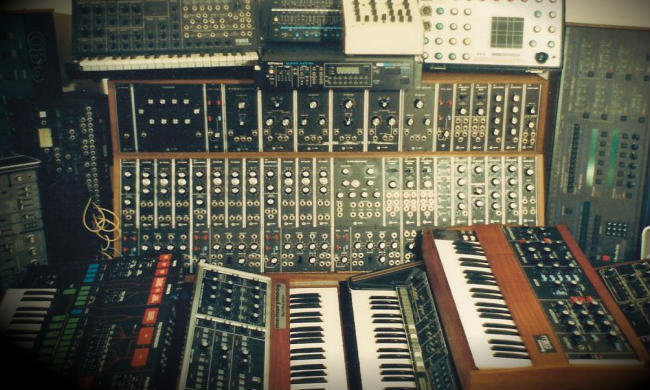
\includegraphics[width=0.45\textwidth]{./Imagenes/Bitmap/foto-sinte.jpg}
\caption[Analog synthesizer.]{Analog synthesizer. {\small Source \citep{SinteFutureMusic}.}}
\label{fig:foto_sinte}
\end{figure}

However, the synthesis landscape changed drastically in the late 1960s with the discovery of Frequency Modulation (FM) Synthesis and, on a massive scale, with the commercialization of the iconic Yamaha DX7 in 1983. 
This technology represented a revolution in the market by allowing the creation of metallic, electric, and bell-like timbres that were acoustically impossible to achieve with the technology of the time. 

Nevertheless, this innovation brought about a significant dilemma: its programming is notoriously counterintuitive. Unlike traditional systems, in FM synthesis a minimal change in a single parameter (such as the modulation index or the frequency of an operator) can completely destroy the harmonic structure of the sound. This extreme parametric sensitivity and the steep learning curve have historically alienated most creators from FM sound design, relegating them to using preconfigured presets.

From a mathematical and acoustic perspective, this problem lies in the lack of injectivity of the synthesis engine: drastically different parameter combinations can generate acoustic results that the human ear perceives as identical, while minuscule adjustments can result in completely opposite sound textures. Consequently, manual sound design becomes a technical barrier that interrupts the artist's creative flow.

This level of technical complexity presents its greatest obstacle in the process known as \textit{Sound Matching} or timbral matching. It is a daily occurrence in the recording studio for a producer to hear a specific sound and wish to replicate it. Performing this task "by ear" with an FM synthesizer is a process of trial and error that can be deeply frustrating. 

\begin{figure}[H]
\centering
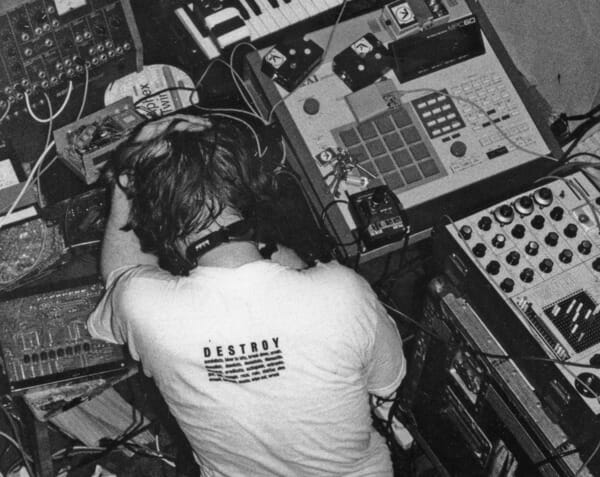
\includegraphics[width=0.45\textwidth]{./Imagenes/Bitmap/aphex-twin.png}
\caption[Aphex Twin programming synthesizers.]{Aphex Twin programming synthesizers. {\small Source \citep{AphexTwinReverb}.}}
\label{fig:aphex_twin}
\end{figure}

Faced with this problem, machine learning, and specifically Deep Learning, present themselves as the ideal bridge between the musician's creative abstraction and the synthesizer's mathematical complexity. By delegating parameter inference to a computational model, the search for the target sound can be automated. To achieve this, the system must be capable of "listening to" and processing the signal in a way that the network can assimilate. By transforming the one-dimensional audio into a \textbf{spectrogram}, the sound is effectively "photographed," adapting the frequencies to a logarithmic scale that closely mimics the human auditory system's perception.

Once the audio is represented as a two-dimensional image, CNNs emerge as the ideal architecture to approach the problem. These networks are designed to extract spatial features and, in the spectrogram domain, are exceptionally precise at "seeing" and classifying the dense timbral and harmonic textures of audio.

All the developed code can be found in our GitHub repository: \\ 
\url{https://github.com/Angelji06/TFG-SoundMatchingFM}

\section{Objectives}
\label{sec:objetivos}

The main objective of the project is to develop a system based on convolutional neural networks capable of automatically estimating the parameters of a frequency modulation (FM) synthesizer from an audio sample, in order to replicate its timbre.  

As specific objectives, the following are established:

\begin{itemize}
    \item \textbf{Dataset generation:} Design and implement a synthesis engine capable of generating a massive dataset of synthetic audios and their corresponding labels (parameters), as well as converting them into tensors.
    \item \textbf{Signal processing:} Establish a signal processing pipeline to transform raw audio into visual representations (spectrograms) suitable for the CNN, applying data transformations and normalizations that maximize its performance.
    \item \textbf{Model development:} Design, train, and optimize various Convolutional Neural Network architectures and loss functions in Python.
    \item \textbf{Psychoacoustic evaluation:} Evaluate the model's performance using parameter error metrics and timbral similarity measures that simulate the perception of the human ear.
    \item \textbf{Interface development:} Develop a system with a functional interface that allows access to all project utilities easily and intuitively.
    \item \textbf{Model study:} Study and compare the use of different spectrogram representations, network architectures, and loss functions.
\end{itemize}

\section{Work Plan}
The development of this Bachelor's Thesis will span from September 2025 to May 2026. The evolution of the project throughout these months will be structured into five clearly defined stages:

\begin{itemize}
    \item \textbf{Phase 1 (September - October): Exploration and proof of concept} \\
    \textbf{Main milestone:} General research stage on Artificial Intelligence applied to music. \\
    During these months, a literature review will be conducted to establish the technical foundations of deep learning and its application to audio. Initial proofs of concept will be developed to evaluate the capabilities of AI applied to synthesizers, experimenting with waveform prediction and spectrogram generation.

    \item \textbf{Phase 2 (November): Project definition, \textit{Sound Matching}, and first functional prototypes} \\
    \textbf{Main milestone:} Establishment of FM \textit{Sound Matching} as the central axis and the first functional prototype. \\
    In this stage, the project will focus on Frequency Modulation (FM) Synthesis and begin generating massive labeled datasets. A first CNN regression model will be trained, and the code architecture will be designed based on Object-Oriented Programming (OOP). Additionally, a basic Graphical User Interface (GUI) will be programmed with the aim of achieving a solid first functional proof of sound matching.

    \item \textbf{Phase 3 (December - February): Scaling complexity and evaluation metrics} \\
    \textbf{Main milestone:} Synthesis improvement and model evaluation. \\
    Once the baseline system is validated, complexity will be added by incorporating new parameters, such as envelopes, into the sound generation. This will require scaling dataset generation and unifying data treatment to ensure consistency in obtaining spectrograms and their proper normalization. Finally, validation metrics will be implemented, and tools to visualize and evaluate the model's results will be developed.

    \item \textbf{Phase 4 (February - April): Architectural optimization and report drafting kickoff} \\
    \textbf{Main milestone:} Deep optimization of the neural network and start of writing. \\
    During these months, the focus will be on developing and refining the final prototype. At the code level, different architectural optimizations in the neural network will be tested, such as using Mel-scale spectrograms and advanced loss functions, while also implementing an FM benchmark for evaluation. In parallel, the writing of the project report will begin, documenting previous developments and the fundamental theoretical basis (Mel scale, MFCC coefficients, etc.).

    \item \textbf{Phase 5 (April - May): Final drafting, definitive model training, and closure} \\
    \textbf{Main milestone:} Completion of the report and training of production models. \\
    With the main code stabilized, programming tasks will be limited to final adjustments oriented toward evaluation and training history logging. The main effort will be allocated to concluding the writing of the report, creating the necessary diagrams, cleaning the code, and preparing execution scripts for different environments (Linux and Windows). Finally, the definitive models will be trained using the computational resources provided by the UCM.
\end{itemize}